\documentclass{amsart}

\usepackage{amsmath,amssymb,amsthm,amsfonts}
\usepackage{tikz,caption}

\theoremstyle{plain}
\newtheorem{theorem}{Theorem}[section]
\newtheorem*{theorem*}{Theorem}
\newtheorem{proposition}[theorem]{Proposition}
\newtheorem{lemma}[theorem]{Lemma}
\newtheorem{corollary}[theorem]{Corollary}

\theoremstyle{definition}
\newtheorem*{definition}{Definition}

\theoremstyle{remark}
\newtheorem{remark}[theorem]{Remark}

\DeclareMathOperator{\im}{im}

\begin{document}

\title[Fold-and-Cut of Simple Closed Curve under Conical Origami]
{Curved Folding and Planar Cutting of \\ Simple Closed Curve on a Conical Origami}

\author[I. Choi]{Ikhan Choi}
\address{Seoul Science High School, 63 Hyehwa-ro Jongno-gu Seoul, South Korea}
\email{ikany@bawi.org}

\subjclass[2010]{53A04,53A05}
\keywords{fold-and-cut theorem, origami, isometric immersion}




\begin{abstract}
The fold-and-cut theorem states that one can find a flat folding of paper, so that 
one complete straight cut on the folding creates any desired polygon. 
We extend this problem to \emph{curved origami} for piecewise $C^1$ simple closed curves.
Many of those curves on paper turn out to be cut by a straight plane 
after we fold the paper into a \emph{conical shape}---the surface consists of half-lines with a common vertex.
Let $\gamma \colon I\to\mathbb{R}^2$ be a piecewise $C^1$ simple closed curve such that there exists a parametrization $\gamma(\psi)=(r(\psi)\cos\psi,r(\psi)\sin\psi)$ on $\psi\in[0,2\pi)$ for a Lipschitz continuous function $r \colon \mathbb{R}\to(0,\infty)$.
We prove that there exists a conical folding of the plane so that $\gamma$ can be cut by a plane on the folding 
if a certain condition on angular total variation holds. 
\end{abstract}



\maketitle

\section{Introduction}%section 1 
%des fold-and-cut theorem, definition of origami
Origami is the art of folding paper, which also often refers to the mathematical study concerned with the paper folding.
The fold-and-cut theorem~\cite{demaine2000folding} states that we can find a flat folding of paper, 
so that one complete straight cut on folding creates any desired polygon.
Inspired by this theorem we suggest in this paper a problem not for flat folding but for \emph{curved folding} embedded in three-dimensional Euclidean space $\mathbb{R}^3$. %revised6
Once you have drawn a curve on a piece of paper, for many of the cases, we can do crumple the paper and cut it with one straight plane to cut out exactly the curve drawn.
To study origami in three-dimensional space, we consider the metric preserving map of ${\Omega\subset\mathbb R}^2$ called an \emph{origami} to model the process of folding the paper.
For the given curve $\gamma \colon I\to\mathbb{R}^2$ and an origami $u \colon \Omega \subset \mathbb{R}^2\to\mathbb{R}^3$, 
the curve $\gamma$ is called a \emph{cut on origami $u$} if there exists a plane $S\subset\mathbb{R}^3$ such that $S\cap\im u=u(\im\gamma)$.
An \emph{origami} is defined as a Lipschitz continuous piecewise $C^1$ map $u \colon \Omega\to\mathbb{R}^3$ for connected set $\Omega\subset\mathbb{R}^2$ such that 
the Jacobian matrix $Du$ is a $3\times 2$ matrix with orthonormal columns for all points of $\Omega\setminus\Sigma_u$, 
where $\Sigma_u\subset\Omega$ is the set of the points at which $u$ is \emph{not} differentiable. 
In addition, to make our model more physically realizable, we require the paper not to intersect itself transversally.
See \cite{dacorogna2008lipschitz}.

%des conical origami
We consider single vertex origami in the curved fold-and-cut problem.
The image of the single vertex origami becomes a (general) cone in $\mathbb{R}^3$, 
a surface generated by a continuously moving half-line cast from a common apex point.
We call the origami $u$ whose image is a cone a \emph{conical origami} when the domain $\Omega$ of $u$ is taken to be the whole plane $\mathbb{R}^2$. %revised2
This paper discusses the existence of the conical origami $u$ such that the given \emph{piecewise $C^1$ simple closed curve} is a cut on $u$.

%des coordinates, proposition
We set up Cartesian coordinates $(x,y)$ on $\mathbb{R}^2$, and cylindrical coordinates $(\rho,\psi,z)$ on $\mathbb{R}^3$.
The origin of $\mathbb{R}^2$ maps to the vertex under the conical origami 
and the $\rho\psi$-plane of $\mathbb{R}^3$ is meant to intersect the image of the origami $u$ 
exactly in $u(\im\gamma)$ where $\gamma$ is the given simple closed curve in $\mathbb{R}^2$.
In Section 2, Proposition~\ref{2.1} 
on piecewise $C^1$ simple closed curves on $\mathbb{R}^2$
describes some necessary conditions for the existence of the conical origami $u$ 
such that the origin of $\mathbb{R}^2$ is the preimage of the vertex and the given piecewise $C^1$ simple closed curve is a cut on $u$.
If such an origami $u$ exists, then the interior of the given simple closed curve $\gamma$ is required to be \emph{star-shaped} 
(there exists a point called the kernel such that any half-line cast from the point intersects $\gamma$ only once).
More precisely, the kernel of the star-shaped curve is the origin.
Namely, the proposition guarantees the existence of a Lipschitz continuous function $r \colon \mathbb{R}\to(0,\infty)$ 
that is periodic with period $2\pi$, such that the piecewise $C^1$ simple closed curve $\gamma$ is parametrized by $\psi\in I=[0,2\pi)$ as $\gamma(\psi)=(r(\psi)\cos\psi,r(\psi)\sin\psi)$.
In this paper, $I$ always denotes the half-open interval $[0,2\pi)$.

%des description of the function Az
Consider the piecewise $C^1$ simple closed curve $\gamma$ in $\mathbb{R}^2$ that is a cut on a certain conical origami.
Then, we have the Lipschitz continuous function $r \colon \mathbb{R}\to(0,\infty)$ that is used to parametrize $\gamma$.
In fact, because the curve $\gamma$ is piecewise $C^1$, the function $r$ is also piecewise $C^1$.
Let $u$ be one of the conical origami on which $\gamma$ is cut, such that $u(O)$ is the vertex of the conical origami and the vertex has cylindrical coordinate $(0,0,z)$ for a positive real number $z$.
For the function $r$, a function $A_z \colon [0,2\pi]\to[0,\infty)$ is defined to be a strictly 
increasing function whose value is equal to the amount of the angle that the point $u(\gamma(\theta))$ has traveled over $\theta\in[0,\psi]$ in the cylindrical coordinates.
In other words, the function $A_z$ is the \emph{total variation} of the angular coordinate of the polar parametrization $u$, so we call $A_z(\psi)$ the \emph{total angular variation} of $u$ up to $\psi$.
Actually the function $A_z$ is independent of $u$, it can be defined only by the function $r$ and a real number $z$.
The function $A_z$ is defined by the following formula: %revised4
\begin{align*}
A_z(\psi):=\int_0^{\psi}\sqrt{\biggl(\frac{r(\theta)}{\sqrt{r(\theta)^2-z^2}}\biggr)^2-\left(\frac{zr'(\theta)}{r(\theta)^2-z^2}\right)^2}\,d\theta.
\end{align*}

%des main result
Our main results are summarized by a part of Theorem~\ref{3.1} as follows:
\begin{theorem*} %Theorem
Let $\gamma$ be a piecewise $C^1$ simple closed curve in $\mathbb{R}^2$ such that there exists a parametrization $\gamma(\psi)=(r(\psi)\cos\psi,r(\psi)\sin\psi)$ on $\psi\in I=[0,2\pi)$ for a Lipschitz continuous function $r \colon \mathbb{R}\to(0,\infty)$ that has period $2\pi$. If
\begin{align}\label{condition}%lab
\sup_{z}\,A_z(2\pi)\ge2\pi,
\end{align}
then there exists a conical origami $u$ such that $\gamma$ is cut on $u$.
\end{theorem*}
\noindent We prove the theorem by directly presenting the conical origami in cylindrical coordinates, that cuts the given simple closed curve.

%des road map
In Section 2, we define new terminologies such as conical origami and give the proposition describing the necessary conditions and existence of the star-shaped parametrization of the given piecewise $C^1$ simple closed curve.
In Section 3, we define the function $A_z$ and the main theorem.
The idea of proof will be also given.
In section 4, we prove the main theorem.






\bigskip

\section{Definition of Conical Origami and Cut}%section 2 
%des
We define a \emph{conical origami} to be a Lipschitz continuous piecewise $C^1$ map for analytic models of paper folding.
For a connected set $\Omega\subset\mathbb{R}^n$ and a piecewise $C^1$ map $f\colon\Omega\to\mathbb{R}^m$, the \emph{singular set} $\Sigma_f\subset\Omega$ of the map $f$ refers to the set of points at which $f$ is not differentiable. %revised1
The map $f$ is $C^1$ on $\Omega\setminus\Sigma_f$, and also, the singular set $\Sigma_f$ is closed in $\Omega$ and each arbitrary compact set in $\Omega$ intersects a finite number of connected components of $\Omega\setminus\Sigma_f$; it is the definition of a piecewise $C^1$ function. %revised1
A conical origami is the origami whose image is a (general) cone with the domain $\mathbb{R}^2$, where the \emph{origami} will be defined as a kind of rigid map that models the paper folding embedded in $\mathbb{R}^3$. %revised2
See \cite{dacorogna2008lipschitz}.
See \cite{arkin2004can,hull1994mathematics,kawasaki1989relation,lang1996computational}
for usual geometric approaches to origami. 

%des
An \emph{origami} is a Lipschitz continuous piecewise $C^1$ map $u\colon\Omega\to\mathbb{R}^3$ such that the Jacobian matrix $Du$ has orthonormal columns 
and transversal self-intersection is excluded.
To make the model more physically realizable, we allow precise overlappings which can be approximated by injective maps, that means, 
$\im u$ can intersect itself tangently. 
For example, the map $u(x,y)=(|x|,y,0)$ is not injective but can be obtained as $k\to\infty$ of the injective maps $u_k(x,y)=(|x|\cos(1/k), y, x\sin(1/k))$, 
which represent the actual folding process along time (see \cite{dacorogna2008lipschitz}).
In this paper, we focus only on \emph{conical origamis}. 


\begin{definition}[Conical Origami]%def %revised2
A Lipschitz continuous piecewise $C^1$ map $u\colon\mathbb{R}^2\to\mathbb{R}^3$ is a \emph{conical origami} if it satisfies the following:
the Jacobian matrix $Du$ has orthonormal columns for all points of $\mathbb{R}^2\setminus\Sigma_u$;
there exists a sequence of maps $u_k\colon\mathbb{R}^2\to\mathbb{R}^3$ that are Lipschitz continuous and injective, such that $u_k\to u$ in the uniform convergence;
the image of $u$ is a cone.

The \emph{vertex of the conical origami $u$} is the vertex point of the image of $u$.
\end{definition}

%des
If the condition that the image of $u$ is a cone is excluded and the domain $\mathbb{R}^2$ is replaced with any connected set $\Omega\subset\mathbb{R}^2$, then the map $u$ is called just an \emph{origami}. %revised2
See \cite{dacorogna2008lipschitz}.

%des
The fold-and-cut theorem states that we can find a flat folding of paper, so that one complete straight cut on folding creates any desired plane graph of cuts made up with straight sides.
Similarly, within three-dimensional space, we ask is there is a (conical) origami map such that a certain planar straight cut on folding creates the given curve, especially \emph{piecewise $C^1$ simple closed curve}, on the unfolded paper.
If there is such an origami $u$, we call the curve a \emph{cut on $u$}.
See \cite{demaine2000folding} for more details on the fold-and-cut theorem. 


\begin{definition}[Cut]%def %revised2
Let $\Omega$ be a connected set in $\mathbb{R}^2$.
A curve $\gamma\colon I\to\Omega$ is a \emph{cut on origami $u\colon\Omega\to\mathbb{R}^3$} if there exists a plane $S\subset\mathbb{R}^3$ such that $S\cap\im u=u(\im \gamma)$.
\end{definition}

%des
We approach the problem about the simple closed curve by a parametrization.
Also the conical origami is parametrized by a metric preserving map whose codomain is presented in cylindrical coordinates.
The cylindrical coordinate system is set up by letting the plane $S$ containing $u(\im\gamma)$ be $\rho\psi$-plane and the preimage of the vertex of $u$ be on the $z$-axis.

%des
The following proposition presents the conditions required for a piecewise $C^1$ simple closed curve to be a cut on a conical origami, regarding the existence of the polar parametrization.
Using the function $r$ defined in the following proposition, we have the polar equation $\rho=r(\psi)$ represent the curve $\gamma$.



\begin{proposition}\label{2.1} %{2.1}
Let $\gamma$ be a piecewise $C^1$ simple closed curve in $\mathbb{R}^2$ and $u$ be a conical origami that has the origin of $\mathbb{R}^2$ as the preimage of its vertex.
If $\gamma$ is a cut on $u$, then there exists a Lipschitz continuous function $r \colon \mathbb{R}\to(0,\infty)$ which has period $2\pi$, such that $\gamma$ has a parametrization $\gamma(\psi)=(r(\psi)\cos\psi,r(\psi)\sin\psi)$ on $\psi\in I=[0,2\pi)$.
\end{proposition}

\begin{proof}
Let $O$ be a point on $\mathbb{R}^2$ such that the point $u(O)$ is the vertex of the conical origami $u$.
First we prove that $\gamma$ is star-shaped with kernel $O$, that is, any half-line cast from $O$ intersects $\gamma$ only once.
Then, we can represent any point on $\gamma$ by $(r(\psi)\cos\psi,r(\psi)\sin\psi)$ for a periodic piecewise $C^1$ function $r \colon \mathbb{R}^2\to(0,\infty)$ with period $2\pi$.
After that, we prove that the function $r$ is Lipschitz continuous if $\gamma$ has the parametrization.
Since the star-shaped curve implies that $r$ is a function on $I$ and positive valued, the proof is complete if we prove that $\gamma$ is star-shaped and the function $r$ is Lipschitz continuous.

We claim that $u(O)$ cannot be in the plane $S$, where the plane $S$ satisfies $S\cap\im u=u(\im\gamma)$.


\begin{figure}%fig 1
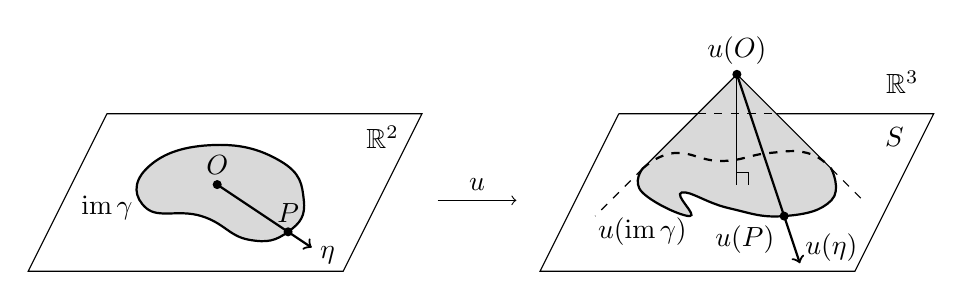
\begin{tikzpicture}
\draw (1,2) -- (0,0) -- (4,0) -- (5,2) -- (1,2);
\draw [thick,fill=gray!30] [-] plot[smooth cycle, tension=.8] coordinates {(3.2,1.4) (2.3,1.6) (1.5,1.3) (1.5,0.8) (2.2,0.7) (2.8,0.4) (3.3,0.5) (3.5,0.9)};
\draw [thick,->] (2.4,1.1) -- (3.6,0.3);

\node at (4.5,1.7) {$\mathbb{R}^2$};
\node [above] at (2.4,1.1) {$O$};
\node at (3.8,0.2) {$\eta$};
\node at (1,0.8) {$\im\gamma$};
\node [above] at (3.3,0.5) {$P$};
\draw [fill] (2.4,1.1) circle (0.05);
\draw [fill] (3.3,0.5) circle (0.05);

\draw [->](5.2,0.9) -- (6.2,0.9);
\node at (5.7,1.1) {$u$};

\draw (7.5,2) -- (6.5,0) -- (10.5,0) -- (11.5,2) -- (7.5,2);
\draw [fill=gray!30] [-] (7.8,1.3) -- (9,2.5) -- (10.2,1.3);
\draw [thick,fill=gray!30] [-] plot[smooth, tension=.8] coordinates {(7.8,1.3) (7.8,1) (8.4,0.7) (8.3,1) (8.9,0.8) (9.6,0.7) (10.2,0.9) (10.2,1.3)};
\draw [thick,dashed] plot[smooth,tension=.8] coordinates {(7.8,1.3) (8.2,1.5) (8.8,1.4) (9.4,1.5) (9.9,1.5) (10.2,1.3)};
\draw [dashed] (8.5,2) -- (9.5,2);
\draw [dashed] (7.8,1.3) -- (7.2,0.7);
\draw [dashed] (10.2,1.3) -- (10.6,0.9);
\draw [thick,->] (9,2.5) -- (9.8,0.1);
\draw (9,2.5) -- (9,1.1);
\draw (9,1.25) -- (9.15,1.25) -- (9.15,1.1);

\node at (11,1.7) {$S$};
\node at (11.1,2.4) {$\mathbb{R}^3$};
\node [above] at (9,2.5) {$u(O)$};
\node [below left] at (9.6,0.7) {$u(P)$};
\node at (10.2,0.3) {$u(\eta)$};
\node at (7.8,0.5) {$u(\im\gamma)$};
\draw [fill] (9,2.5) circle (0.05);
\draw [fill] (9.6,0.7) circle (0.05);
\end{tikzpicture}
\caption{The point $u(O)$ cannot be in the plane $S$ and the curve $\gamma$ is star-shaped.}
\end{figure}


\begin{figure}%fig 2
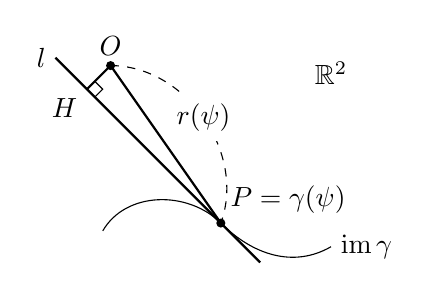
\begin{tikzpicture}
\draw (0.4,0.4) to [out=60,in=135] (1.9,0.5) to [out=315,in=210] (3.3,0.2);
\draw [thick] (-0.2,2.6) -- (2.4,0);
\draw [thick] (0.2,2.2) -- (0.5,2.5) -- (1.9,0.5);
\draw (0.3,2.3) -- (0.4,2.2) -- (0.3,2.1);
\draw [dashed] (0.5,2.5) to [bend left=55] node [fill=white] {$r(\psi)$} (1.9,0.5);

\node [above right] at (1.9,0.5) {$P=\gamma(\psi)$};
\node [above] at (0.5,2.5) {$O$};
\node [left] at (-0.2,2.6) {$l$};
\node at (3.3,2.4) {$\mathbb{R}^2$};
\node [right] at (3.3,0.2) {$\im\gamma$};
\node [below left] at (0.2,2.2) {$H$};
\draw [fill] (1.9,0.5) circle (0.05);
\draw [fill] (0.5,2.5) circle (0.05);
\end{tikzpicture}
\caption{The function $r$ is Lipschitz continuous.}
\end{figure}


For the proof, 
assume that $u(O)$ is in the plane $S$.
For a point $P\ne O$ which is on the curve $\gamma$, we have $u(P)\in S$.
If we let $\eta$ be a half-line on $\mathbb{R}^2$ such that $u(\eta)$ cast from $u(O)$ and passing through the point $u(P)$, then the plane $S$ contains $u(\eta)$ because $u(O)$ is in $S$.
The image $(\im u)$ also contains the half-line $u(\eta)$ because $(\im u)$ is a conical surface.
Since $u(\eta)$ is included in both $S$ and $(\im u)$, we obtain $u(\eta)\subset u(\im\gamma)$ from the relation $S\cap\im u=u(\im \gamma)$.
So, the curve $u(\gamma)$ is unbounded and it is a contradiction for $\gamma$ to be a closed curve.
Therefore $u(O)$ cannot be in the plane $S$.

(\emph{star-shapedness})
Assume that $\gamma$ is not star-shaped.
If a half-line $\eta$ cast from $O$ intersects $\im\gamma$ more than once, the image $u(\eta)$ also intersects $u(\gamma)$ more than once.
Since $S\supset u(\im\gamma)\supset u(\im\gamma)\cap u(\eta)$ and the cardinality of $u(\im\gamma)\cap u(\eta)$ is greater than one, $S$ contains the half line $u(\eta)$ and also the point $O$.
By the same argument for the previous claim, 
each half-line $\eta$ cast from $O$ intersects $\im\gamma$ at most once.
If there is a half-line cast from $O$ that does not meet $\im\gamma$, the point $O$ should be in the interior of the simple closed curve $\gamma$ and there exists a half-line which intersects $\im\gamma$ more than twice.
Therefore all of the half-lines cast form $O$ intersects $\im\gamma$ only once, and the $\gamma$ is star-shaped.

(\emph{Lipschitz continuity})
For a point $P$ on the curve $\gamma$, there exists a piecewise $C^1$ function $r \colon \mathbb{R}\to(0,\infty)$ such that we have $P=\gamma(\psi)=(r(\psi)\cos\psi,r(\psi)\sin\psi)$ on $\psi\in I$ because $\gamma$ is star-shaped and the kernel is $O$.
Let $l$ be a tangent line at a point $P$, and $H$ be the foot of the perpendicular from $O$ to $l$.
From $\frac{r'(\psi)}{r(\psi)}=\tan\left(\frac{\pi}2-\angle OPH\right)$, we have the length of the line segment $OH$ as follows:
\begin{align*}
OH(\psi)=r(\psi)\sin\angle OPH=\frac{r(\psi)^2}{\sqrt{r(\psi)^2+r'(\psi)^2}}.
\end{align*}
Let $z$ be the distance between the point $u(O)$ and the plane $S$ in $\mathbb{R}^3$.
Since $S$ contains $u(l)$, we have $0\le z\le OH(\psi)$ for all $\psi$.
If the derivative $r$ is unbounded, then the value of $OH(\psi)$ can be arbitrarily small.
So we have $z=0$, it implies that $u(O)$ is on the plane $S$.
The function $r$ is piecewise $C^1$ and the derivative of $r$ is bounded, hence the function $r$ is Lipschitz continuous.
\end{proof}

%des
Note that the function $r$ has positive lower bound, since $O$ is in the interior of $\gamma$.
In Theorem~\ref{3.1}, a concrete construction of the conical origami is presented on the cylindrical coordinates for the given piecewise $C^1$ simple closed curve, that has the star shaped parametrization with Lipschitz continuous function $r$ and satisfies the condition (\ref{condition}).
In fact, the coordinate system on $\mathbb{R}^2$ and the preimage of the vertex of the conical origami is given in advance.









\bigskip



\section{The Main Theorem and The Idea of Proof}%section 3 
%des
For a given piecewise $C^1$ simple closed curve $\gamma$ that satisfies the condition (\ref{condition}) and the assumption of 
Proposition~\ref{2.1}, we propose a map $u \colon \mathbb{R}^2\to\mathbb{R}^3$ in Theorem~\ref{3.1}.
Let $r \colon \mathbb{R}\to(0,\infty)$ be a Lipschitz continuous function with period $2\pi$ such that $\gamma$ has a parametrization $\gamma(\psi)=(r(\psi)\cos\psi,r(\psi)\sin\psi)$ on $\psi\in I=[0,2\pi)$.
We introduce \emph{total angular variation} $A_z(\psi)$ for the definition of the map $u$.
After stating Theorem~\ref{3.1}, we are going to describe our plan to prove the theorem.  
We prove that this map $u$ is a conical origami and $\gamma$ is cut on $u$ in Section~4.

%des
For the moment, assume that $u$ is a conical origami such that $u(O)$ is the vertex of the conical origami and it has cylindrical coordinate $(0,0,z)$ for a positive real number $z$.
Suppose that the given curve $\gamma$ is a cut on $u$.
We suggest a function $A_z \colon [0,2\pi]\to[0,\infty)$ defined as a strictly increasing function whose value is equal to the amount of the angle that the point $u(\gamma(\theta))$ has traveled over $\theta\in[0,\psi]$ in the cylindrical coordinates.
In other words, the function $A_z$ is the total variation of the angular coordinate of the polar parametrization $u$, so we call $A_z(\psi)$ the \emph{total angular variation} of $u$ up to $\psi$.
If the image $u(\im \gamma)$ is also star-shaped, then $A_z(\psi)$ is the angular coordinate of $u(\gamma(\psi))$.

\begin{figure}%fig 3
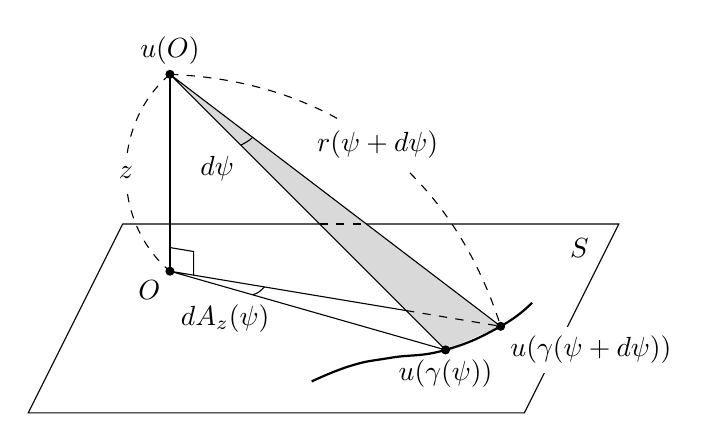
\begin{tikzpicture}
\draw (-0.6,0.6) -- (-1.8,-1.8) -- (4.5,-1.8) -- (5.7,0.6) -- (-0.6,0.6);
\draw (3,-0.5) -- (0,0) -- (3.5,-1);
\draw (0,0) -- (0,2.5);
\draw [fill=gray!30] (3.5,-1) -- (0,2.5) --(4.2,-0.7);
\draw [dashed] (3,-0.5) -- (4.2,-0.7);
\draw [dashed] (1.9,0.6) -- (2.5,0.6);
\draw (0.3,-0.05) -- (0.3,0.25) -- (0,0.3);
\draw [thick] plot[smooth, tension=.8] coordinates {(1.8,-1.4) (2.3,-1.2) (2.8,-1.1) (3.5,-1) (4.2,-0.7) (4.6,-0.4)};
\draw (0.9,1.6) to [out=30,in=225] (1.05,1.7);
\draw (1.05,-0.3) to [out=15,in=225] (1.2,-0.2);
\draw [dashed] (0,2.5) to [bend left=35] node [fill=white] {$r(\psi+d\psi)$} (4.2,-0.7);
\draw [dashed] (0,2.5) to [bend right=50] node [fill=white] {$z$} (0,0);

\node at (5.2,0.3) {$S$};
\node [below left] at (0,0) {$O$};
\node [above] at (0,2.5) {$u(O)$};
\node [below] at (3.5,-1) {$u(\gamma(\psi))$};
\node [below right,fill=white] at (4.2,-0.7) {$u(\gamma(\psi+d\psi))$};
\node at (0.6,1.3) {$d\psi$};
\node at (0.7,-0.6) {$dA_z(\psi)$};
\draw [fill] (3.5,-1) circle (0.05);
\draw [fill] (4.2,-0.7) circle (0.05);
\draw [fill] (0,0) circle (0.05);
\draw [fill] (0,2.5) circle (0.05);
\end{tikzpicture}
\caption{The infinitesimal triangle and its projection to the plane.}
\end{figure}

%des
Consider a infinitesimal triangle constructed by three points $u(\gamma(\psi+d\psi))$, $u(O)$, and $u(\gamma(\psi))$.
Recall that the range of the map $u\circ\gamma$ belongs to $\rho\psi$-plane, which is the plane $S$ in the definition of a cut.
By projection of this triangle to $\rho\psi$-plane, we say that the infinitesimal value of the total angular variation $dA_z(\psi)$ denotes the size of the angle constructed by $u(\gamma(\psi+d\psi))$, $O$, and $u(\gamma(\psi))$.
If this infinitesimal angle was integrated from $0$ to $\psi$, then the value would be same with $A_z(\psi)$.
Since $u$ preserves the metric, the infinitesimal angle $d\psi$ denotes the angle $dA_z(\psi)$ before the projection.
Actually the function $A_z$ is independent of $u$, it can be defined only by the function $r$ and a positive real number $z$.

%des
The function $A_z$ can be calculated through the projection of the angle mapped by $u$ on the $\rho\psi$-plane.
Let $z$ be the altitude of the vertex of the conical origami.
By the law of cosines, we have a relation between the infinitesimal $d\psi$ and $dA_z(\psi)$ as follows:
\begin{align*}
&r(\psi)^2+r(\psi+d\psi)^2-2r(\psi)r(\psi+d\psi)\cos d\psi\,
\\&\qquad\qquad\qquad=\,\left(r(\psi)^2-z^2\right)+\left(r(\psi+d\psi)^2-z^2\right)
\\&\qquad\qquad\qquad\qquad-2\sqrt{r(\psi)^2-z^2}\sqrt{r(\psi+d\psi)^2-z^2}\cos dA_z(\psi).
\end{align*}
By the half-angle formula for sine and some calculations, we obtain the square of the derivative of $A_z$:
\begin{align*}
\left(\frac{dA_z(\psi)}{d\psi}\right)^2=\biggl(\frac{r(\psi)}{\sqrt{r(\psi)^2-z^2}}\biggr)^2-\left(\frac{zr'(\psi)}{r(\psi)^2-z^2}\right)^2
\end{align*}
where $r'$ denotes the derivative of $r$.
Note that $A_z$ can be determined only by $r$ and $z$.
Since the sign of the derivative of $A_z$ with respect to $\psi$ cannot be determined in here, we define the angular coordinate of $u$ as the integral of the product of $dA_z/d\psi$ and either $1$ or $(-1)$ in Theorem~\ref{3.1}.

%des
Before giving the definition of the function $A_z$, the domain of $z$ is defined as the open interval $U_r$ that depends on the function $r$. 
If the nonnegative real number $z$ does not belong to $U_r$, then the image of $u$ is the plane if $z=0$; there exist a point such that $A_z$ is not strictly increasing if $z=\sup U_r$; the integrand of the integral $A_z$ is not real number if $z>\sup U_r$.


\begin{definition}%def
Let $\gamma$ be a piecewise $C^1$ simple closed curve in $\mathbb{R}^2$ that has a parametrization $\gamma(\psi)=(r(\psi)\cos\psi,r(\psi)\sin\psi)$ on $\psi\in I=[0,2\pi)$, for a Lipschitz continuous function $r \colon \mathbb{R}\to(0,\infty)$ with period $2\pi$.
The open interval $U_r$ is defined as follows:
\begin{align*}
U_r:=\left(\;0\,,\;\inf_{\psi\in I\setminus\Sigma_r}\frac{r(\psi)^2}{\sqrt{r(\psi)^2+r'(\psi)^2}}\,\right),
\end{align*}
where $r'$ denotes the derivative of the function $r$ and $\Sigma_r$ denotes the singular set.
For each $z\in U_r$, an injective function  $A_z \colon [0,2\pi]\to[0,\infty)$ is defined by the following integral:
\begin{align*}
A_z(\psi):=\int_0^{\psi}\sqrt{\biggl(\frac{r(\theta)}{\sqrt{r(\theta)^2-z^2}}\biggr)^2-\left(\frac{zr'(\theta)}{r(\theta)^2-z^2}\right)^2}\,d\theta.
\end{align*}
The value $A_z(\psi)$ is called the \emph{total angular variation} of $u$ up to $\psi$.
\end{definition}


%des
In particular, we define $A_0(\psi)$ to be equal to $\psi$.
Because the total angular variation $A_z$ does not allude the sign of the infinitesimal change of the angular coordinate, something to indicate the sign is required.
For a subset $\kappa$ of the interval $I$, let $A_z^{\kappa}(\psi)$ be a abbreviation of the integral
\begin{align*}
A_z^{\kappa}(\psi)=\int_0^{\psi}(-1)^{\bold{1}_{\kappa}(\theta)}A'_z(\theta)\,d\theta,
\end{align*}
where $A'_z$ denotes the derivative of $A_z$ with respect to $\psi$ and $\bold{1}_{\kappa}$ is the indicator function of $\kappa$.
The value of $A_z^{\kappa}(\psi)$ can represent the exact angular coordinate of a conical origami in cylindrical coordinates.
If $\psi$ belongs to $\kappa$, then the infinitesimal change of the angular coordinate becomes negative. 

%des
Since the derivative of $A_z$ is positive, the function $A_z$ is strictly increasing in $\psi$ and thereby it has an inverse function.
We will often use the property that $A_z$ is strictly increasing.
The curve $\gamma$ is piecewise $C^1$, so the function $r$ is $C^1$ on the set $\mathbb{R}\setminus\Sigma_r$.
The derivative $r'$ is bounded since the function $r$ is Lipschitz continuous, and the function $r$ has a positive lower bound.
So, the open interval $U_r$ is non-empty.




\begin{theorem}\label{3.1} %{3.1}
Let $r \colon \mathbb{R}\to(0,\infty)$ be a Lipschitz continuous function with period $2\pi$ and $\gamma$ be a piecewise $C^1$ simple closed curve in $\mathbb{R}^2$ that has a parametrization $\gamma(\psi)=(r(\psi)\cos\psi,r(\psi)\sin\psi)$ on $\psi\in I=[0,2\pi)$.  
If
\begin{align*}
\sup_{z\in U_r}\,A_z(2\pi)\ge2\pi, \tag{\ref{condition}}
\end{align*}
then there exist a closed interval $\kappa\subset I$ and a real number $z\in U_r$ such that a map $u \colon \mathbb{R}^2\to\mathbb{R}^3$ is a conical origami and $\gamma$ is a cut on $u$;
the map $u$ is defined as follows:
\begin{align}\label{origami}%lab
u(\rho,\psi)_{polar}=\left(\;\rho\sqrt{1-\frac{z^2}{r(\psi)^2}}\,,
\;A_z^{\kappa}(\psi)\,,
\;z\left(1-\frac{\rho}{r(\psi)}\right)\,\right)_{cylindrical}.
\end{align}
\end{theorem}

%des %revised3
The condition (\ref{condition}) is required.
For an example let $r(\psi)=96+\arccos(\cos100\psi)$, then $|r'(\psi)|>r(\psi)$ for all $\psi$, so $A'_z(\psi)<1$ for all $z$ and $\psi$; since $A'_z(\psi)<1$ if and only if $r(\psi)^2-z^2<r'(\psi)^2$.
For this example we have
\begin{align*}
A_z(2\pi)=\int_0^{2\pi}A'_z(\psi)\,d\psi<\int_0^{2\pi}\,d\psi=2\pi
\end{align*}
for all $z\in U_r$.

%des
The proof of Theorem~\ref{3.1} will be given at the end of Section 4.
Note that the map $u$ defined in Theorem~\ref{3.1} as (\ref{origami}) depends only on $r$ and $\kappa$ and $z$, because we defined $A_z$ only with $r$ and $z$.
Let $u$ be the map defined in Theorem~\ref{3.1} as (\ref{origami}).
The altitude of a point $u(\rho\cos\psi,\rho\sin\psi)=u(\rho,\psi)_{polar}$ in cylindrical coordinate is $0$ if and only if $\rho=r(\psi)$, that is, the point $(\rho\cos\psi,\rho\sin\psi)$ is on the curve $\gamma$.
So we get $S\cap\im u=u(\im \gamma)$ where $S$ is the plane $z=0$, and the curve $\gamma$ is a cut on $u$ if $u$ is an origami.

%des
Recall the definition of the conical origami.
To prove that the map $u$ is a conical origami, we have to show that the following four propositions are true:
\begin{itemize}
\item The Jacobian matrix $Du$ has orthonormal columns for all points of $\mathbb{R}^2\setminus\Sigma_u$.
\item The image of $u$ is a cone.
\item There exists a sequence of maps $u_k$ that are injective and uniformly converges to $u$.
\item The maps $u_k$ and $u$ are Lipschitz continuous, and $u$ is piecewise $C^1$.
\end{itemize}
We give the proof of Theorem~\ref{3.1} throughout Section 4.
For the map $u$ defined in Theorem~\ref{3.1}, Theorem~\ref{4.1} shows that $u$ preserves metric and Proposition~\ref{4.2} shows that the image of $u$ is a cone.
The proof of the other two conditions for conical origami is divided into two cases: the function $r$ is a constant function or not.
The case of the nonconstant function is treated in Theorem~\ref{4.3},~\ref{4.4},\and~\ref{4.5}; the case of the constant function is treated in Theorem~\ref{4.6}.

%des
In the case of nonconstant function, it is proved that we can find an injective $u$, so that we can let $u_k$ be same with $u$.
For an interval $\kappa=[\alpha,\beta]\subset I$ and a real number $z\in U_r$, the following three conditions play an important role in the proof.
\begin{enumerate}
\item both $2A_z(\alpha)-A_z(\beta)$ and $2A_z(\beta)-A_z(\alpha)$ belong to the interval $[0,A_z(2\pi))$;
\item the function $r$ is strictly increasing over the interval 
\begin{align*}
J=[A_z^{-1}(2A_z(\alpha)-A_z(\beta)),A_z^{-1}(2A_z(\beta)-A_z(\alpha))];
\end{align*}
\item the value of $A_z^{\kappa}(2\pi)$ is equal to $2\pi$.
\end{enumerate}
Recall that the map $u$ is determined by only $\kappa$ and $z$ if the curve $\gamma$ and the function $r$ were already given.
Theorem~\ref{4.3} shows that there exist an interval $\kappa=[\alpha,\beta]\subset I$ and a real number $z\in U_r$ satisfying the three conditions if $r$ is nonconstant.
Theorem~\ref{4.4} shows that the map $u$ is injective if the three conditions are satisfied.
Theorem~\ref{4.5} shows that the map $u$ is Lipschitz continuous and piecewise $C^1$ if the third condition of the three conditions is satisfied.



\begin{figure}[h]%fig 4
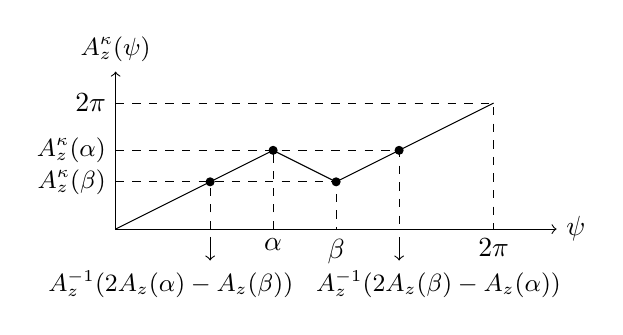
\begin{tikzpicture}
\draw [<->] (0,2) -- (0,0) -- (5.6,0);
\draw (0,0) -- (2,1) -- (2.8,0.6) -- (4.8,1.6);
\draw [dashed] (0,0.6) -- (2.8,0.6) -- (2.8,0);
\draw [dashed] (0,1) -- (3.6,1) -- (3.6,0);
\draw [dashed] (0,1.6) -- (4.8,1.6) -- (4.8,0);
\draw [dashed] (1.2,0) -- (1.2,0.6);
\draw [dashed] (2,0) -- (2,1);
\draw [->] (1.2,-0.1) -- (1.2,-0.4);
\draw [->] (3.6,-0.1) -- (3.6,-0.4);

\node [right] at (5.6,0) {$\psi$};
\node [above] at (0,2) {\small$A_z^{\kappa}(\psi)$};
\node at (0.7,-0.7) {\small$A_z^{-1}(2A_z(\alpha)-A_z(\beta))$};
\node [below] at (2,0) {$\alpha$};
\node [below] at (2.8,0) {$\beta$};
\node at (4.1,-0.7) {\small$A_z^{-1}(2A_z(\beta)-A_z(\alpha))$};
\node [below] at (4.8,0) {$2\pi$};
\node [left] at (0,0.6) {\small$A_z^{\kappa}(\beta)$};
\node [left] at (0,1) {\small$A_z^{\kappa}(\alpha)$};
\node [left] at (0,1.6) {$2\pi$};
\draw [fill] (1.2,0.6) circle (0.05);
\draw [fill] (2,1) circle (0.05);
\draw [fill] (2.8,0.6) circle (0.05);
\draw [fill] (3.6,1) circle (0.05);
\end{tikzpicture}
\caption{The rough shape of the graph of the function $A_z^{\kappa}$ for a closed interval $\kappa=[\alpha,\beta]$.}
\end{figure}


%des
Condition~(1) ensures the existence of the interval $J$ in Condition~(2), where $A_z^{-1}$ denotes the inverse function of $A_z$.
The interval $J$ in Condition~(2) is used to prove that $u$ is injective.
To prove the injectivity of $u$, it is enough to show that the curve $u\circ\gamma$ is simple because the image of $u$ is a cone.
A point $u(\gamma(\psi))$ traces the curve $u\circ\gamma$ counter-clockwise, but clockwise when $\psi$ is in the interval $\kappa$.
So, the curve $u\circ\gamma$ can intersects itself only if the angular coordinate of $u$ is between $A_z^{\kappa}(\beta)$ and $A_z^{\kappa}(\alpha)$.
From the definition of $A_z^{\kappa}$, we have
\begin{align*}
A_z^{\kappa}\Bigl(A_z^{-1}\bigl(2A_z(\alpha)-A_z(\beta)\bigr)\Bigr)=A_z^{\kappa}(\beta)\,,\; A_z^{\kappa}\Bigl(A_z^{-1}\bigl(2A_z(\beta)-A_z(\alpha)\bigr)\Bigr)=A_z^{\kappa}(\alpha).
\end{align*}
It implies that we do not have to check whether $u\circ\gamma$ intersects itself for $\psi\notin J$.
The condition that $r$ is strictly increasing over $J$ that $u\circ\gamma$ is injective.
The details of this idea will be presented rigorously in Theorem~\ref{4.4}.
Condition~(3) is necessary for $u$ to be continuous because the map $u$ is given on the polar coordinates.
By these conditions, we can conclude that there exists an conical origami $u$ on which the given simple closed curve $\gamma$ is a cut if the function $r$ is not a constant function.

%des
If the function $r$ is constant, the curve $\gamma$ is a circle such that the center is the origin of $\mathbb{R}^2$ and the radius is $r$.
Intuitively, we can see any circle is a cut on a certain conical origami, which is folded like filter paper.
In this case, the sequence of maps $u_k$ is required to be different from $u$ since the limit point $u$ is not injective, so we define a sequence $u_k$ separately from $u$.
Theorem~\ref{4.6} shows that a filter-paper-like folding satisfies the third and fourth condition to be a conical origami.

\begin{figure}%fig 5
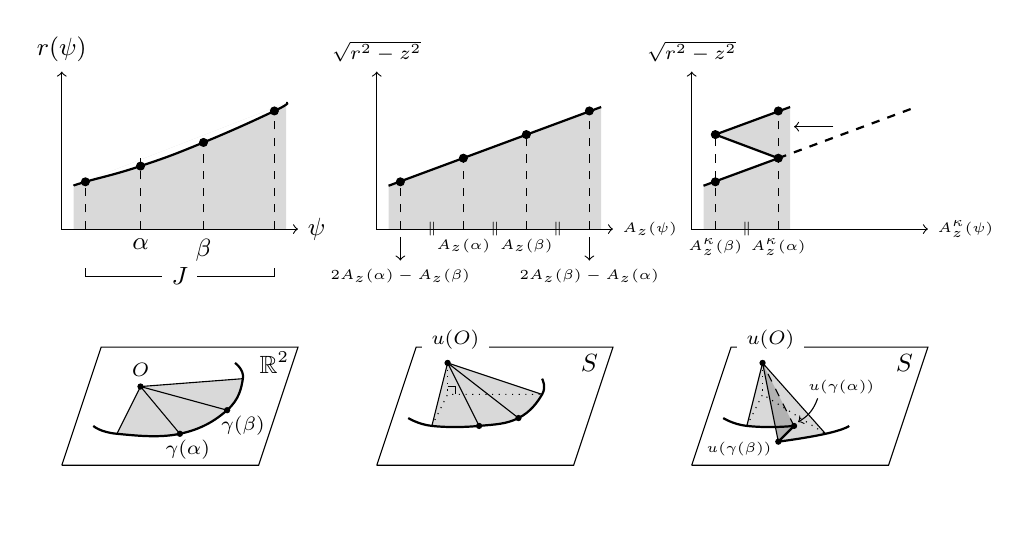
\begin{tikzpicture}
\fill [gray!30] (0.15,0) -- (2.85,0) -- (2.85,1.6) -- (0.15,0.55) -- (0.15,0);
\draw [<->] (0,2) -- (0,0) --(3,0);
\draw [thick,fill=white] plot[smooth,tension=.8] coordinates{(0.15,0.55) (0.3,0.6) (1,0.8) (1.8,1.1) (2.7,1.5) (2.85,1.6)};
\draw [dashed] (0.3,0) -- (0.3,0.6);
\draw [dashed] (1,0) -- (1,0.9);
\draw [dashed] (1.8,0) -- (1.8,1.2);
\draw [dashed] (2.7,0) -- (2.7,1.5);
\draw (0.3,-0.5) -- (0.3,-0.6) to node [fill=white] {\small$J$} (2.7,-0.6) -- (2.7,-0.5);

\node [above] at (0,2) {\small$r(\psi)$};
\node [right] at (3,0) {\small$\psi$};
\node [below] at (1,0) {\small$\alpha$};
\node [below] at (1.8,0) {\small$\beta$};
\draw [fill] (0.3,0.6) circle (0.05);
\draw [fill] (1,0.8) circle (0.05);
\draw [fill] (1.8,1.1) circle (0.05);
\draw [fill] (2.7,1.5) circle (0.05);


\fill [gray!30] (4.15,0) -- (6.85,0) -- (6.85,1.55) -- (4.15,0.55) -- (4.15,0);
\draw [<->] (4,2) -- (4,0) --(7,0);
\draw [thick] (4.15,0.55) -- (6.85,1.55);
\draw [dashed] (4.3,0) -- (4.3,0.6);
\draw [dashed] (5.1,0) -- (5.1,0.9);
\draw [dashed] (5.9,0) -- (5.9,1.2);
\draw [dashed] (6.7,0) -- (6.7,1.5);
\draw [->] (4.3,-0.1) -- (4.3,-0.4);
\draw [->] (6.7,-0.1) -- (6.7,-0.4);

\node [above] at (4,2) {\scriptsize$\sqrt{r^2-z^2}$};
\node [right] at (7,0) {\tiny$A_z(\psi)$};
\node [below] at (5.1,0) {\tiny$A_z(\alpha)$};
\node [below] at (5.9,0) {\tiny$A_z(\beta)$};
\node at (4.3,-0.6) {\tiny$2A_z(\alpha)-A_z(\beta)$};
\node at (6.7,-0.6) {\tiny$2A_z(\beta)-A_z(\alpha)$};
\draw [fill] (4.3,0.6) circle (0.05);
\draw [fill] (5.1,0.9) circle (0.05);
\draw [fill] (5.9,1.2) circle (0.05);
\draw [fill] (6.7,1.5) circle (0.05);


\fill [gray!30] (8.15,0) -- (9.25,0) -- (9.25,1.55) -- (8.3,1.2) -- (9.1,0.9) -- (8.15,0.55) -- (8.15,0);
\draw [<->] (8,2) -- (8,0) --(11,0);
\draw [thick] (8.15,0.55) -- (9.1,0.9) -- (8.3,1.2) -- (9.25,1.55);
\draw [thick, dashed] (9.1,0.9) --(10.85,1.55);
\draw [->] (9.8,1.3) -- (9.3,1.3);
\draw [dashed] (8.3,0) -- (8.3,1.2);
\draw [dashed] (9.1,0) -- (9.1,1.5);

\node [above] at (8,2) {\scriptsize$\sqrt{r^2-z^2}$};
\node [right] at (11,0) {\tiny$A_z^{\kappa}(\psi)$};
\node [below] at (9.1,0) {\tiny$A_z^{\kappa}(\alpha)$};
\node [below] at (8.3,0) {\tiny$A_z^{\kappa}(\beta)$};
\draw [fill] (8.3,0.6) circle (0.05);
\draw [fill] (9.1,0.9) circle (0.05);
\draw [fill] (8.3,1.2) circle (0.05);
\draw [fill] (9.1,1.5) circle (0.05);

\node at (4.7,0) {\tiny$\|$};
\node at (5.5,0) {\tiny$\|$};
\node at (6.3,0) {\tiny$\|$};
\node at (8.7,0) {\tiny$\|$};

%------------\\

\begin{scope}
\clip (0.4,-3.2) -- (1,-2) -- (3.6,-1.8);
\fill [gray!30] plot[smooth,tension=.7] coordinates {(0.4,-2.5) (0.7,-2.6) (1.5,-2.6) (2.1,-2.3) (2.3,-1.9) (2.2,-1.7)};
\end{scope}
\draw (0,-3) -- (2.5,-3) -- (3,-1.5) -- (0.5,-1.5) -- (0,-3);
\draw [fill=gray!30] (0.7,-2.6) -- (1,-2) -- (2.3,-1.9);
\draw [thick] plot[smooth,tension=.7] coordinates {(0.4,-2.5) (0.7,-2.6) (1.5,-2.6) (2.1,-2.3) (2.3,-1.9) (2.2,-1.7)};
\draw (2.1,-2.3) -- (1,-2) -- (1.5,-2.6);

\node at (2.7,-1.7) {\small$\mathbb{R}^2$};
\node [above] at (1,-2) {\scriptsize$O$};
\node at (1.6,-2.8) {\scriptsize$\gamma(\alpha)$};
\node at (2.3,-2.5) {\scriptsize$\gamma(\beta)$};
\fill (1,-2) circle (0.04);
\fill (2.1,-2.3) circle (0.04);
\fill (1.5,-2.6) circle (0.04);


\begin{scope}
\clip (4.5,-3.3) -- (4.9,-1.7) -- (7.3,-2.5);
\fill [gray!30] plot[smooth,tension=.7] coordinates {(4.4,-2.4) (4.7,-2.5) (5.3,-2.5) (5.8,-2.4) (6.1,-2.1) (6.1,-1.9)};
\end{scope}
\draw (4,-3) -- (6.5,-3) -- (7,-1.5) -- (4.5,-1.5) -- (4,-3);
\draw [fill=gray!30] (4.7,-2.5) -- (4.9,-1.7) -- (6.1,-2.1);
\draw [dotted] (4.9,-1.7) -- (4.9,-2.1);
\draw [dotted] (4.7,-2.5) -- (4.9,-2.1) -- (6.1,-2.1);
\draw (5.3,-2.5) -- (4.9,-1.7) -- (5.8,-2.4);
\draw [thick] plot[smooth,tension=.7] coordinates {(4.4,-2.4) (4.7,-2.5) (5.3,-2.5) (5.8,-2.4) (6.1,-2.1) (6.1,-1.9)};
\draw (4.9,-2) -- (5,-2) -- (5,-2.1);

\node at (6.7,-1.7) {\small$S$};
\node [fill=white] at (5,-1.4) {\scriptsize$u(O)$};
\fill (4.9,-1.7) circle (0.04);
\fill (5.3,-2.5) circle (0.04);
\fill (5.8,-2.4) circle (0.04);


\begin{scope}
\clip (9.7,-3.3) -- (8.9,-1.7) -- (8.5,-3.3);
\fill [gray!30] plot[smooth,tension=.7] coordinates {(8.4,-2.4) (8.7,-2.5) (9.3,-2.5) (9.8,-2.4)};
\end{scope}
\begin{scope}
\clip (9.3,-3.7) -- (8.9,-1.7) -- (10.5,-3.5);
\fill [gray!30] plot[smooth,tension=1] coordinates {(9.1,-2.7) (9.7,-2.6) (10,-2.5)};
\end{scope}
\fill [gray!30] (8.9,-1.7) -- (8.7,-2.5) -- (9.3,-2.5) -- (9.1,-2.7) -- (9.7,-2.6) -- (8.9,-1.7);
\fill [gray!60] (9.1,-2.7) -- (8.9,-1.7) -- (9.3,-2.5);
\draw (8,-3) -- (10.5,-3) -- (11,-1.5) -- (8.5,-1.5) -- (8,-3);
\draw (8.7,-2.5) -- (8.9,-1.7) -- (9.7,-2.6);
\draw [dashed] (9.3,-2.5) -- (8.9,-1.7);
\draw [dotted] (8.7,-2.5) -- (8.9,-2.1) -- (9.7,-2.6);
\draw [dotted] (8.9,-1.7) -- (8.9,-2.1);
\draw (8.9,-1.7) -- (9.1,-2.7);
\begin{scope}
\clip (9.7,-3.3) -- (8.9,-1.7) -- (7.9,-3.1);
\draw [thick] plot[smooth,tension=.7] coordinates {(8.4,-2.4) (8.7,-2.5) (9.3,-2.5) (9.8,-2.4)};
\end{scope}
\draw [thick] (9.1,-2.7) -- (9.3,-2.5);
\draw [thick] plot[smooth,tension=1] coordinates {(9.1,-2.7) (9.7,-2.6) (10,-2.5)};

\node at (10.7,-1.7) {\small$S$};
\node [fill=white] at (9,-1.4) {\scriptsize$u(O)$};
\draw [<-] (9.35,-2.45) to [out=30,in=250] (9.6,-2.15);
\node at (9.9,-2) {\tiny$u(\gamma(\alpha))$};
\node at (8.6,-2.8) {\tiny$u(\gamma(\beta))$};
\fill (8.9,-1.7) circle (0.04);
\fill (9.1,-2.7) circle (0.04);
\fill (9.3,-2.5) circle (0.04);
\end{tikzpicture}
\caption{If the function $r$ is strictly increasing over $J$, then the map $u$ is injective.}
\end{figure}




\bigskip

\section{The proof of The Main Theorem}%section4 
% proof : metric preserving
\begin{theorem}\label{4.1} %{4.1}
Let $r \colon \mathbb{R}\to(0,\infty)$ be a Lipschitz-continuous piecewise-$C^1$ function.
For a closed interval $\kappa=[\alpha,\beta]\subset I=[0,2\pi)$ and a real number $z\in U_r$, let $u \colon \mathbb{R}^2\to\mathbb{R}^3$ be the map defined in Theorem~\ref{3.1} (\ref{origami}).
The map $u$ is a local isometric immersion on $\mathbb{R}^2\setminus\Sigma_u$, that is, the Jacobian matrix $Du$ has orthonormal columns for all points of $\mathbb{R}^2\setminus\Sigma_u$.
\end{theorem}

\begin{proof}%pf
The partial derivatives of $u$ in cylindrical coordinates are
\begin{align*}
\frac{\partial u}{\partial\rho}=\left(\;\sqrt{1-\frac{z^2}{r(\psi)^2}}\,,\;0\,,\;-\frac{z}{r(\psi)}\,\right),
\end{align*}
and
\begin{align*}
\frac{\partial u}{\partial\psi}=\left(\frac{\rho z^2r'(\psi)}{r(\psi)^2\sqrt{r(\psi)^2-z^2}}\,,\;(-1)^{\bold{1}_{\kappa}(\psi)}A'_z(\psi)\,,\;\frac{\rho zr'(\psi)}{r(\psi)^2}\right),
\end{align*}
where the derivative of the function $A_z$ is
\begin{align*}
A'_z(\psi)=\sqrt{\biggl(\frac{r(\psi)}{\sqrt{r(\psi)^2-z^2}}\biggr)^2-\left(\frac{zr'(\psi)}{r(\psi)^2-z^2}\right)^2}.
\end{align*}

The metric $g$ on the image of $u$ is
\begin{align*}
g=\begin{pmatrix}1&0&0\\0&\rho^2\left(1- {z^2}/{r(\psi)^2}\right)&0\\0&0&1\end{pmatrix}
\end{align*}
because the codomain of $u$ was given in the cylindrical coordinate system.
Then, we have a calculation of the first fundamental form with the inner product in the metric $g$ as follows:
\begin{align*}
E=\left\langle\frac{\partial u}{\partial\rho},\frac{\partial u}{\partial\rho}\right\rangle=1\,,\;
F=\left\langle\frac{\partial u}{\partial\rho},\frac{\partial u}{\partial\psi}\right\rangle=0\,,\;
G=\left\langle\frac{\partial u}{\partial\psi},\frac{\partial u}{\partial\psi}\right\rangle=\rho^2\,.
\end{align*}
It is same with the metric of polar coordinates, hence $u$ is a local isometric immersion at all points at which $u$ is differentiable.
\end{proof}





% proof : cone
\begin{proposition}\label{4.2} %{4.2}
Let $r \colon \mathbb{R}\to(0,\infty)$ be a Lipschitz-continuous piecewise-$C^1$ function. 
For a closed interval $\kappa=[\alpha,\beta]\subset I=[0,2\pi)$ and a real number $z\in U_r$, let $u \colon \mathbb{R}^2\to\mathbb{R}^3$ be the map defined in Theorem~\ref{3.1} as (\ref{origami}).
The image of $u$ is a cone, not embedded in a plane, such that $u(O)$ is vertex of the cone.
\end{proposition}

\begin{proof}%pf
The equality $\partial^2u/\partial\rho^2=0$ implies $u$ is linear in $\rho$.
The image $u(O)$ is $(0,0,z)$ regardless of $\psi$.
It means that the image of $u$ is a cone, not embedded in a plane, because $z>0$. 
\end{proof}







% proof : nonconst -> exists, st. three conditions
\begin{theorem}\label{4.3} %{4.3}
Let $r \colon \mathbb{R}\to(0,\infty)$ be a Lipschitz continuous function with period $2\pi$ and $\gamma$ be a piecewise $C^1$ simple closed curve in $\mathbb{R}^2$ that has a parametrization $\gamma(\psi)=(r(\psi)\cos\psi,r(\psi)\sin\psi)$ on $\psi\in I=[0,2\pi)$. 
If $r$ is not a constant function and $\sup_{z\in U_r}A_z(2\pi)\ge2\pi$, then there exists an interval $\kappa=[\alpha,\beta]\subset I$ and a real number $z\in U_r$ that satisfy:
\begin{enumerate}
\item both $2A_z(\alpha)-A_z(\beta)$ and $2A_z(\beta)-A_z(\alpha)$ belong to the interval $[0,A_z(2\pi))$;
\item the function $r$ is strictly increasing over the interval 
\begin{align*} 
J=[A_z^{-1}(2A_z(\alpha)-A_z(\beta)),A_z^{-1}(2A_z(\beta)-A_z(\alpha))];
\end{align*} 
\item the value of $A_z^{\kappa}(2\pi)$ is equal to $2\pi$.
\end{enumerate}
\end{theorem}

\begin{proof}%pf
First assume that there is $z$ such that $A_z(2\pi)=2\pi$.
For this $z$, let $\alpha=\beta$.
Then, we can say that $r$ is strictly increasing over $J=[\alpha,\beta]=\{\alpha\}$ since $2A_z(\alpha)-A_z(\beta)=2A_z(\beta)-A_z(\alpha)=\alpha=\beta$.
Furthermore, the measure of $\kappa=[\alpha,\beta]$ is $0$, so we get
\begin{align*}
A_z(2\pi)=A_z^{\kappa}(2\pi)=2\pi.
\end{align*}
The set $\kappa=\{\alpha\}$ and this $z$ satisfy the three conditions.

Otherwise if there is no $z$ such that $A_z(2\pi)=2\pi$, then $A_z(2\pi)>2\pi$ for all $z\in U_r$ because $A_z$ is continuous and
\begin{align*}
\sup_{z\in U_r}\,A_z(2\pi)\ge2\pi.
\end{align*}
Throughout the rest of the proof, assume that $A_z(2\pi)>2\pi$ for all $z$.

Suppose that the function $r$ is strictly increasing on a positive length interval $[a,b]\subset I$.
Because the function $r$ is piecewise $C^1$ and periodic, such an interval $[a,b]$ exists.
Let $\alpha_0(t)$ and $\beta_0(t)$ be a function defined on $U_r$ by:
\begin{align*}
\alpha_0(t)=A_t^{-1}\left(\frac23A_t(a)+\frac13A_t(b)\right),\beta_0(t)=A_t^{-1}\left(\frac13A_t(a)+\frac23A_t(b)\right).
\end{align*}
From $A_t(a)<A_t(b)$, we get $\alpha_0(t)<\beta_0(t)$ for a sufficiently small $t$.
Let $z_0$ be a real number in $U_r$ satisfying
\begin{align*}
\sup_{t<z_0}\,\alpha_0(t)<\inf_{t<z_0}\,\beta_0(t).
\end{align*}
Let us define $\kappa$ as an interval $[\alpha,\beta]\subset\left[\sup_{t<z_0}\,\alpha_0(t),\inf_{t<z_0}\,\beta_0(t)\right]$ such that
\begin{align*}
0<\beta-\alpha<\frac{A_{z_0}(2\pi)-2\pi}{2\sup_{\psi\in I\setminus\Sigma_r}\,A'_{z_0}(\psi)}.
\end{align*}

For the fixed $\kappa$, consider the value of $A_z^{\kappa}(2\pi)$ as a function of $z$.
This function is equal to $A_z(2\pi)-2\bigl(A_z(\beta)-A_z(\alpha)\bigr)$ and continuous with respect to $z$.
By letting $z=z_0$, we obtain
\begin{align*}
A_{z_0}^{\kappa}(2\pi)
&= A_{z_0}(2\pi)-2\int_{\alpha}^{\beta}A'_{z_0}(\theta)\,d\theta \\
&\ge A_{z_0}(2\pi)-2(\beta-\alpha)\sup_{\psi\in I\setminus\Sigma_r}\,A'_{z_0}(\psi) >2\pi.
\end{align*}
On the other hand, letting $z=0$, we get
\begin{align*}
A_0^{\kappa}(2\pi)=2\pi-2(\beta-\alpha)<2\pi.
\end{align*}
By the intermediate value theorem, there exists $z\in(0,z_0)$ satisfying the third condition.
We will show that these $\kappa$ and $z$ satisfy the other two conditions.

From the definition of $\kappa$, We get
\begin{align*}
\alpha_0(z)\le\sup_{t<z_0}\,\alpha_0(t)\le\alpha\,,\;\beta\le\inf_{t<z_0}\,\beta_0(t)\le\beta_0(z).
\end{align*}
It implies that $A_z(\alpha_0(z))\le A_z(\alpha)$, $A_z(\beta)\le A_z(\beta_0(z))$ and
\begin{align*}
A_z(a)=2A_z(\alpha_0(z))-A_z(\beta_0(z))&\le2A_z(\alpha)-A_z(\beta)\\
\le2A_z(\beta)-A_z(\alpha)&\le2A_z(\beta_0(z))-A_z(\alpha_0(z))=A_z(b).
\end{align*}
Since $2A_z(\alpha)-A_z(\beta)$ and $2A_z(\beta)-A_z(\alpha)$ belong to the interval $[A_z(a),A_z(b)]$, the two values are in the range of $A_z$.
Also, we have the interval $J=[A_z^{-1}(2A_z(\alpha)-A_z(\beta)),A_z^{-1}(2A_z(\beta)-A_z(\alpha))]$ be a subset of $[a,b]$, which the function $r$ is strictly increasing on.
Hence, the first and second conditions are satisfied.
\end{proof}







%proof : three condition -> injectivity
\begin{theorem}\label{4.4} %{4.4}
Let $r \colon \mathbb{R}\to(0,\infty)$ be a Lipschitz continuous function with period $2\pi$ and $\gamma$ be a piecewise $C^1$ simple closed curve in $\mathbb{R}^2$ that has a parametrization $\gamma(\psi)=(r(\psi)\cos\psi,r(\psi)\sin\psi)$ on $\psi\in I=[0,2\pi)$. 
For a closed interval $\kappa=[\alpha,\beta]\subset I$ and a real number $z\in U_r$, let $u \colon \mathbb{R}^2\to\mathbb{R}^3$ be the map defined in Theorem~\ref{3.1} as (\ref{origami}).
The map $u$ is injective if $\kappa$ and $z$ satisfy the following conditions:
\begin{enumerate}
\item both $2A_z(\alpha)-A_z(\beta)$ and $2A_z(\beta)-A_z(\alpha)$ belong to the interval $[0,A_z(2\pi))$;
\item the function $r$ is strictly increasing over the interval
\begin{align*}
J=[A_z^{-1}(2A_z(\alpha)-A_z(\beta)),A_z^{-1}(2A_z(\beta)-A_z(\alpha))];
\end{align*}
\item the value of $A_z^{\kappa}(2\pi)$ is equal to $2\pi$.
\end{enumerate}
\end{theorem}

\begin{proof}%pf
Assume that $u$ is not injective, that is, there exist two distinct points $(\rho_1,\psi_1),(\rho_2,\psi_2)$ on polar coordinates such that $u(\rho_1\cos\psi_1,\rho_1\sin\psi_1)=u(\rho_2\cos\psi_2,\rho_2\sin\psi_2)$.
From
\begin{align*}
\rho_1\sqrt{1-\frac{z^2}{r(\psi_1)^2}}=\rho_2\sqrt{1-\frac{z^2}{r(\psi_2)^2}}\,,\;
z\left(1-\frac{\rho_1}{r(\psi_1)}\right)=z\left(1-\frac{\rho_2}{r(\psi_2)}\right),
\end{align*}
we obtain $\rho_1=\rho_2$ and $r(\psi_1)=r(\psi_2)$; suppose that $0\le\psi_1<\psi_2<2\pi$.
Also, we have $A_z^{\kappa}(\psi_1)\equiv A_z^{\kappa}(\psi_2)\pmod{2\pi}$.
The function $A_z^{\kappa} \colon [0,2\pi]\to[0,\infty)$ has local minimums at $\psi=0,\beta$, and local maximums at $\psi=\alpha,2\pi$.
By the third condition, we have
\begin{align*}
A_z^{\kappa}(2\pi)=A_z(2\pi)-2\bigl(A_z(\beta)-A_z(\alpha)\bigr)=2\pi,
\end{align*}
and by the first condition, the following inequalities hold:
\begin{gather*}
A_z^{\kappa}(\alpha)=A_z(\alpha)=2\pi-\Bigl(A_z(2\pi)-\bigl(2A_z(\beta)-A_z(\alpha)\bigr)\Bigr)<2\pi,\\
A_z^{\kappa}(\beta)=A_z(\alpha)-\bigl(A_z(\beta)-A_z(\alpha)\bigr)\ge0.
\end{gather*}
Therefore, the value of $A_z^{\kappa}(\psi)$ for $\psi\in I$ belongs to the interval $I$ and we obtain
\begin{align*}
A_z^{\kappa}(\psi_1)=A_z^{\kappa}(\psi_2).
\end{align*}

If we suppose $[\psi_1,\psi_2]\cap\kappa=\varnothing$, then $A_z^{\kappa}(\psi_2)-A_z^{\kappa}(\psi_1)=A_z(\psi_2)-A_z(\psi_1)>0$.
So we get $\psi_2\ge\alpha$ and $\psi_1\le\beta$.
Since $A_z^{\kappa}(\alpha)$ and $A_z^{\kappa}(\beta)$ are the local extrema of $A_z^{\kappa}$, we have
\begin{align*}
A_z^{\kappa}(\alpha)-A_z^{\kappa}(\psi_1)=|A_z(\alpha)-A_z(\psi_1)|\ge A_z(\alpha)-A_z(\psi_1)
\end{align*}
and
\begin{align*}
A_z^{\kappa}(\psi_2)-A_z^{\kappa}(\alpha)\ge A_z^{\kappa}(\beta)-A_z^{\kappa}(\alpha)=-\bigl(A_z(\beta)-A_z(\alpha)\bigr).
\end{align*}
Combining these two inequalities, we obtain $A_z(\psi_1)\ge 2A_z(\alpha)-A_z(\beta)$ by
\begin{align*}
0=A_z^{\kappa}(\psi_2)-A_z^{\kappa}(\psi_1)\ge2A_z(\alpha)-A_z(\beta)-A_z(\psi_1).
\end{align*}
Similarly, we also obtain $A_z(\psi_2)\le2A_z(\beta)-A_z(\alpha)$. These imply that $\psi_1$ and $\psi_2$ belong to the interval $J=[A_z^{-1}\bigl(2A_z(\alpha)-A_z(\beta)\bigr),A_z^{-1}\bigl(2A_z(\beta)-A_z(\alpha)\bigr)]$.
Because the function $r$ is strictly increasing over $J$, $r(\psi_1)$ cannot be equal to $r(\psi_2)$.
The assumption that $u$ is not injective leads to a contradiction. 
\end{proof}







%proof : three conditions -> Lc,pC1
\begin{theorem}\label{4.5} %{4.5}
Let $r \colon \mathbb{R}\to(0,\infty)$ be a Lipschitz continuous function with period $2\pi$ and $\gamma$ be a piecewise $C^1$ simple closed curve in $\mathbb{R}^2$ that has a parametrization $\gamma(\psi)=(r(\psi)\cos\psi,r(\psi)\sin\psi)$ on $\psi\in I=[0,2\pi)$. 
For a closed interval $\kappa\subset I$ and a real number $z\in U_r$, let $u \colon \mathbb{R}^2\to\mathbb{R}^3$ be the map defined in Theorem~\ref{3.1} as (\ref{origami}).
The map $u$ is Lipschitz continuous and piecewise $C^1$ if $A_z^{\kappa}(2\pi)=2\pi$.
\end{theorem}

\begin{proof}
If we prove the continuity of $u$, the Lipschitz continuity is proved since each component of the derivatives of $u$ is bounded for each variable.
Also, $u$ is piecewise $C^1$ since each component of $u$ is piecewise $C^1$.
Let us prove the continuity of $u$.

Since each component of $u$ is continuous, it is suffice to prove continuity in polar coordinates, 
that is, to check that the following conditions hold:
\begin{align*}
\begin{cases}
\text{for all $\psi$}&,\displaystyle{\lim_{\rho\to0}}\,u(\rho,\psi)=u(0,\psi) \\
\text{for all $\rho$}&,u(\rho,0)=u(\rho,2\pi)
\end{cases}
\end{align*}
where $u(\rho,\psi)$ is defined on a polar coordinate system.
Recall that the map $u$ is defined as
\begin{align*}
u(\rho,\psi)_{polar}=\left(\;\rho\sqrt{1-\frac{z^2}{r(\psi)^2}}\,,
\;A_z^{\kappa}(\psi)\,,
\;z\left(1-\frac{\rho}{r(\psi)}\right)\,\right)_{cylindrical}.
\end{align*}
The first condition is clearly true.
The second condition is also true because $r(2\pi)=r(0)$ implies that the radial and axial components of $u(\rho,0)_{polar}$ and $u(\rho,2\pi)_{polar}$ are respectively same, and the difference of the angular coordinates $A_z^{\kappa}(2\pi)-A_z^{\kappa}(0)$, which is equal to $2\pi$, is an integer multiple of $2\pi$.
Therefore, the map $u$ is continuous.
\end{proof}




%des
In Theorem~\ref{4.6}, we deal with the case that the function $r$ is a constant function.
Since the derivative of $r$ is $0$, we have $U_r=(0,r)$ and $A'_z=r/\sqrt{r^2-z^2}$.
For the simple statement of the proof, the notation $A'$ still denotes $r/\sqrt{r^2-z^2}$ for given $z$.

\begin{figure}%fig 6
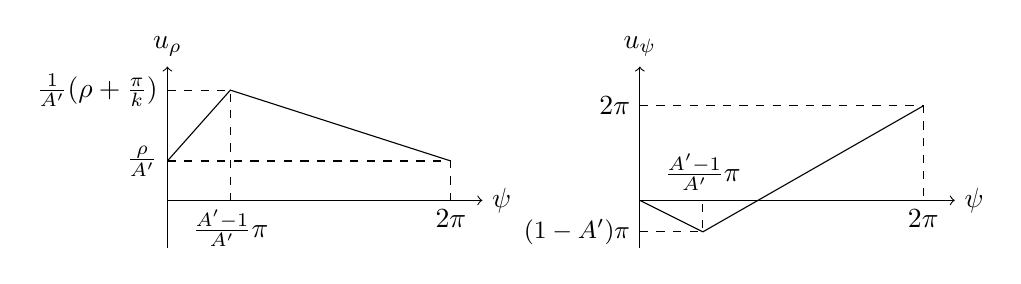
\begin{tikzpicture}
\draw [->] (0,-0.6) -- (0,1.7);
\draw [->] (0,0) -- (4,0);
\draw (0,0.5) -- (0.8,1.4) -- (3.6,0.5);
\draw [dashed] (0,1.4) -- (0.8,1.4) -- (0.8,0);
\draw [dashed] (0,0.5) -- (3.6,0.5) -- (3.6,0);

\node [right] at (4,0) {$\psi$};
\node [above] at (0,1.7) {$u_{\rho}$};
\node [below] at (3.6,0) {$2\pi$};
\node [below] at (0.8,0) {$\frac{A'-1}{A'}\pi$};
\node [left] at (0,0.5) {$\frac{\rho}{A'}$};
\node [left] at (0,1.4) {$\frac1{A'}(\rho+\frac{\pi}k)$};


\draw [->] (6,-0.6) -- (6,1.7);
\draw [->] (6,0) -- (10,0);
\draw (6,0) -- (6.8,-0.4) -- (9.6,1.2);
\draw [dashed] (6,-0.4) -- (6.8,-0.4) --(6.8,0);
\draw [dashed] (6,1.2) -- (9.6,1.2) -- (9.6,0);

\node [right] at (10,0) {$\psi$};
\node [above] at (6,1.7) {$u_{\psi}$};
\node [below] at (9.6,0) {$2\pi$};
\node [left] at (6,1.2) {$2\pi$};
\node [above] at (6.8,0) {$\frac{A'-1}{A'}\pi$};
\node [left] at (6,-0.4) {\small$(1-A')\pi$};
\end{tikzpicture}
\caption{The radial and angular coordinates of $u_k$.}
\end{figure}

% constant r
\begin{theorem}\label{4.6} %{4.6}
Let $r$ be a positive real number and $\gamma$ be a circle parametrized by angle; $\gamma(\psi)=(r\cos\psi,r\sin\psi)$ on $\psi\in I=[0,2\pi)$.
There exists a closed interval $\kappa$ for every $z\in U_r$ such that the curve $\gamma$ is a cut on $u \colon \mathbb{R}^2\to\mathbb{R}^3$, which is defined in Theorem~\ref{3.1} as (\ref{origami}).
\end{theorem}

\begin{proof}
Let $z$ be a real number in $(0,r)$ and $A'=r/\sqrt{r^2-z^2}$.
Let $\kappa=\bigl[0,\frac{A'-1}{A'}\pi\bigr]$.
Let $u_k \colon \mathbb{R}^2\to\mathbb{R}^3$ be a sequence of maps such that: 
\begin{align*}
u_k(\rho,\psi)_{polar} &=\left(\;\frac{\rho}{A'}+\frac1k\cdot\frac{\psi}{A'-1}\,,\;-A'\psi\,,\;z\left(1-\frac{\rho}{r}\right)\,\right)_{cylindrical}
\ \text{for }\psi\in\kappa; 
\end{align*} 
and
\begin{align*} 
u_k(\rho,\psi)_{polar} &=\left(\;\frac{\rho}{A'}+\frac1k\cdot\frac{2\pi-\psi}{A'+1}\,,\;A'\psi-2\pi(A'-1)\,,\;z\left(1-\frac{\rho}{r}\right)\,\right)_{cylindrical}
\end{align*}
for $ \psi\in[0,2\pi]\setminus\kappa$.

The sequence $u_k$ converges uniformly to a map $u$ as $k\to\infty$, which coincides with what we define in Theorem~\ref{3.1} (\ref{origami}) for the interval $\kappa$.
So, the Jacobian matrix $Du$ has orthonormal columns for all points of $\mathbb{R}^2\setminus\Sigma_u$ by Theorem~\ref{4.1}, and the image of $u$ is a cone by Proposition~\ref{4.2}.
Assume that 
there exist distinct points $(\rho_1,\psi_1),(\rho_2,\psi_2)$ on polar coordinates such that $u_k(\rho_1\cos\psi_1,\rho_1\sin\psi_1)=u_k(\rho_2\cos\psi_2,\rho_2\sin\psi_2)$.
Then, we obtain $\rho_1=\rho_2$, and $0\le\psi_1\le\frac{A'-1}{A'}\pi<\psi_2<2\pi$ without loss of generality.
Solving the equation
\begin{align*}
\frac{\psi_1}{A'-1}=\frac{2\pi-\psi_2}{A'+1},\quad-A'\psi_1=A'\psi_2-2\pi(A'-1)
\end{align*}
we have $\psi_1=\psi_2=\frac{A'-1}{A'}\pi$. Therefore the map $u_k$ is injective.

From $u_k(\rho,0)_{polar}=u_k(\rho,2\pi)_{polar}$, we can also prove that $u_k$ and $u$ are Lipschitz continuous and piecewise $C^1$ with the same logic with Theorem~\ref{4.5}.
Therefore, the map $u$ is a conical origami if $\kappa=\bigl[0,\frac{A'-1}{A'}\pi\bigr]$.

Let $S$ be the plane $z=0$ in the cylindrical coordinate system.
A point $u(\rho\cos\psi,\rho\sin\psi)$ is in $S$ if and only if $\rho=r$, which means the point is on the circle $\gamma$.
So, we have $S\cap\im u=u(\im\gamma)$.
Hence, the circle $\gamma$ is cut on the conical origami $u$.
\end{proof}




\begin{proof}[Proof of Theorem~\ref{3.1}]%pf
By Theorem~\ref{4.6}, Theorem~\ref{3.1} is true if the function $r$ is a constant function.

If the function $r$ is not a constant function,
by Theorem~\ref{4.1} and Proposition~\ref{4.2}, the Jacobian matrix $Du$ has orthonormal columns for all points of $\mathbb{R}^2\setminus\Sigma_u$ and the image of $u$ is a cone.
There exist a closed interval $\kappa\subset I$ and a real number $z\in U_r$ such that:
\begin{enumerate}
\item both $2A_z(\alpha)-A_z(\beta)$ and $2A_z(\beta)-A_z(\alpha)$ belong to the interval $[0,A_z(2\pi))$;
\item the function $r$ is strictly increasing over the interval
\begin{align*}
J=[A_z^{-1}(2A_z(\alpha)-A_z(\beta)),A_z^{-1}(2A_z(\beta)-A_z(\alpha))];
\end{align*}
\item the value of $A_z^{\kappa}(2\pi)$ is equal to $2\pi$
\end{enumerate}
by Theorem~\ref{4.3}.
By Theorem~\ref{4.4} and~\ref{4.5}, the map $u$ is injective, Lipschitz continuous, and piecewise $C^1$.
If we let $u_k$ be a sequence of maps such that $u_k=u$ for all positive integer $k$, then $u_k$ uniformly converges to $u$ and the map $u$ is a conical origami.
Let $S$ be the plane $z=0$ in the cylindrical coordinate system.
A point $u(\rho\cos\psi,\rho\sin\psi)$ is in $S$ if and only if $\rho=r(\psi)$, which means the point is on the curve $\gamma$.
So, we have $S\cap\im u=u(\im\gamma)$.
The curve $\gamma$ is a cut on the conical origami $u$ for the $\kappa$ and $z$ satisfying the above three conditions.

Hence, the statement of Theorem~\ref{3.1} is true.
\end{proof}

\section*{Acknowledgement}
This work is done in Student Research Program of Seoul Science High School. 
The author thank Dr.~Won Taek Song for his support and advice 
throughout the research work and preparation of the manuscript. 


\bibliographystyle{plain}
\bibliography{cut}





\end{document}














